\documentclass[10pt,twocolumn,letterpaper]{article}

\usepackage{cvpr}
\usepackage{times}
\usepackage{epsfig}
\usepackage{graphicx}
\usepackage{amsmath}
\usepackage{amssymb}

% Include other packages here, before hyperref.

% If you comment hyperref and then uncomment it, you should delete
% egpaper.aux before re-running latex.  (Or just hit 'q' on the first latex
% run, let it finish, and you should be clear).
%\usepackage[pagebackref=true,breaklinks=true,letterpaper=true,colorlinks,bookmarks=false]{hyperref}

\cvprfinalcopy % *** Uncomment this line for the final submission

%\def\cvprPaperID{****} % *** Enter the CVPR Paper ID here
%\def\httilde{\mbox{\tt\raisebox{-.5ex}{\symbol{126}}}}

% Pages are numbered in submission mode, and unnumbered in camera-ready
\ifcvprfinal\pagestyle{empty}\fi
\begin{document}

%%%%%%%%% TITLE
\title{Breadboard to Schematic}

\author{Catherine Olsson \\
MIT\\
{\tt\small catherio@mit.edu}
% For a paper whose authors are all at the same institution,
% omit the following lines up until the closing ``}''.
% Additional authors and addresses can be added with ``\and'',
% just like the second author.
% To save space, use either the email address or home page, not both
\and
Michele Pratusevich\\
MIT\\
{\tt\small mprat@mit.edu}
}

\maketitle
\thispagestyle{empty}

%%%%%%%%% ABSTRACT
\begin{abstract}

TODO: Write the abstract.

\end{abstract}

%%%%%%%%% BODY TEXT
\section{Introduction}

Breadboards are an important tool for do-it-yourself hardware designers to
quickly test circuit systems. They are easy to assemble, easy to change, and
easy to test, so are the tool of choice for the first prototype of many
hobbyists and students. A programmatically-drawn, or more likely hand-drawn,
schematic diagram is used to prototype the circuit board, but if the circuit is
going to be used for high-speed, low-noise, or multiple-production
applications, a printed circuit board (PCB) is much more desirable than a
breadboard. Our approach to solve this problem was a vision-based tool designed
to go from a picture of a breadboard circuit to a file written in a PCB-ready
format given by Eagle. Through a variety of approaches, we found the task too
large and have implemented pieces of the full pipeline. Them main goal of the
project was to transform the information about the circuit that we had in image
form (pixel representation) to a different more general representation
(component representation). 

%-------------------------------------------------------------------------

\section{Related Work}

\subsection{Properties of Breadboards}

When solving vision-based problems, it is critical to know your system
properties to better develop algorithms customized to the strengths and
weaknesses of a particular application. Photos of breadboards have a number of
interesting properties that can be useful in segmentation, identification, and
restructuring tasks. A number of visually-interesting properties are listed here:
\begin{itemize}
\item A single component on a breadboard, such as a wire, LED, or chip is often a single color. 
\item The colors of the various components are often easily visually distinguishable. 
\item The breadboard is often square with the image. 
\item The breadboard, when not covered with components, has a black checkered pattern of holes in it. 
\item The breadboard color is relatively constant over the entire breadboard, except for the holes.
\item Breadboards follow a specific connectivity pattern. In Figure \ref{fig:board}, each column (not including the ttop two and bottom two rows) can be considered a single connection. The middle gap in the square holes is a break in the connection for each column, so there are five total holes connected to one connection in each of the columns. The top two and bottom rwo rows are connected horizontally into a single connection. Typically, one denotes a voltage of $+5$ volts and one denotes \verb|GND|, or $0$ volts. 
\end{itemize}

\begin{figure}[t]
\begin{center}
   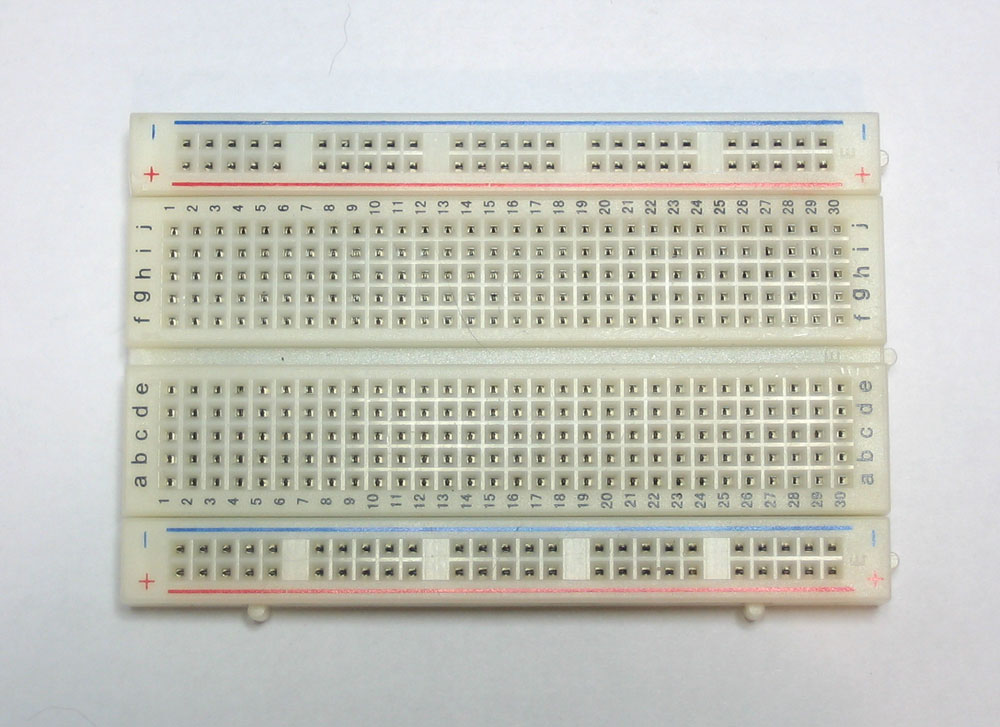
\includegraphics[width=0.8\linewidth]{imgs/breadboard.jpg}
\end{center}
   \caption{A breadboard oriented like those oriented in images that we can process}
\label{fig:board}
\end{figure}


\subsection{Schematic-drawing Software}

The Eagle program, developed by CADSoft, is a free schematic and PCB-drawing
software that translates schematics into a PCB-ready format. The Eagle file
format is a type of XML, which makes it easy to programmatically update from an
image. Eagle PCB and schematic diagrams are based off of the same language, so
drawing a schematic in Eagle is sufficient to computing the full PCB. 

%-------------------------------------------------------------------------
\section{The Approach}

The problem of translating information from a picture of a circuit to a
PCB-friendly file format has two main steps. First, the components must be
identified in the image, and second, the components must be placed in a virtual
grid representation independent of their relation in the image. 

For our implementation we chose to use python and it's Tkinter, PIL, SciPy, and
Numpy packages for ease of implementation, user interface, and speed. 

%-------------------------------------------------------------------------
\subsection{Segmentation into Circuit Components}

\subsubsection{Color Following}

As a first step to tackling the component segmentation problem, we took
advantage of the natural segmentation in a breadboard picture according to
color. Components on a breadboard are different colors that are localized in
one location, so to take advantage of this, we developed an algorithm that
``grows'' a component based on a given color pixel. A seed color is given to
the algorithm and added to an active set of pixels. For each neighbor of each
pixel in the active set, the decision is made whether that pixel is in the
component if the pixel does not change the running RGB color-average of all the
pixels current in the component. If a pixel is added to a component, it is then
also added to the active set and the algorithm continues.     

The main problem with this algorithm is that it is highly dependent on the seed
pixel to the image. If a pixel is chosen that is too dark for example, the
running average that the algorithm will calculate will be off from the actual
running average of the color of the component, so the algorithm will return
incorrect results.   

\subsubsection{k-Means Clustering}

TODO

\subsection{Occlusion Handling}

A problem with breadboard circuits is often that components (most often wires)
are occluded from each other. This is a critical issue that in any finalized
version of a product like this needs to be addressed. Because we ran into other
issues with our approach, we were not able to effectively solve the occlusion
problem.  

\subsection{Virtual Grid Representation}

The next component of the project involved translating the component data into
a schematic. Knowing all the pixel locations that make up a component, we
calculate the end pixel positions of each component rounded to the nearest
$10$. Because components are aligned to the hole-grid that is present on the
breadboard, the calculated endpoints of the components can be used to place
components on a grid in the schematic. The rounded values for the $x$ and $y$
coordinates are used to place the components into their XML representations
into the schematic. 

After all components are identified and represented in their XML formats, a new
file is constructed with the proper sschematic-XML information.    

%-------------------------------------------------------------------------
\section{Results}

\subsection{Comparing Color-following and k-Means Clustering}

TODO

\subsection{Limitations}

One limitation of our product as we've written it is that it can only handle
breadboard circuits that are oriented horizontally as shown above in Figure
\ref{fig:board}. This is because connectivity properties of the breadboard are
geometry-dependent, and our program automatically assumes a particular
orientation for the breadboard to infer connectivity.  

%-------------------------------------------------------------------------
\section{Future Work}

TODO: automatically identify components

%-------------------------------------------------------------------------
\section{Conclusion}

TODO

{\small
\bibliographystyle{ieee}
\bibliography{egbib}
}

\end{document}
